% =============================================================================
%  SOUTENANCE ENSAE (stage de fin d'études, MS Actuariat), novembre 2026
%  Support Beamer, 15 minutes d'exposé. Version courte du support complet
%  (soutenance_institut.tex) : deux diapositives passent en annexe de questions. Forme reprise de la présentation de
%  Lucas Offroy (navigation par section, une idée par diapositive, figures
%  légendées) ; contenu et consignes d'Hugo Rapior du 22 octobre 2026.
%
%  Les nombres viennent du rapport ou des compléments après dépôt explicitement cités.
%  Le contrôle numérique repère les concordances sans valider leur interprétation. Les exemples dessinés
%  (diapositives de démarche) sont étiquetés « illustratif ».
%
%  Compilation, depuis ce dossier :
%     ..\..\..\outils\tectonic\tectonic.exe -X compile soutenance_ensae.tex
% =============================================================================
\documentclass[aspectratio=169,10pt,t]{beamer}
\usepackage{fontspec}
\usepackage[french]{babel}
\frenchsetup{StandardItemizeEnv=true,StandardEnumerateEnv=true}
\usepackage{amsmath,amssymb}
\usepackage{booktabs,array,tabularx,colortbl,multirow}
\usepackage{tikz}
\usepackage{adjustbox}
\usetikzlibrary{arrows.meta,positioning,calc,fit,backgrounds,shapes.geometric}
\usepackage{xspace}
\graphicspath{{../../vasicek_lab/figures/}{../figures_soutenance/}{../../../memoire/logos/}{../charte_nexialog/}}

% ----------------------------------------------------------------- couleurs (gabarit Nexialog)
\definecolor{ardoise}{HTML}{223E55}
\definecolor{acier}{HTML}{435B6E}
\definecolor{encre}{HTML}{122738}
\definecolor{gris}{HTML}{595959}
\definecolor{accent}{HTML}{B10031}
\definecolor{clair}{HTML}{F2F2F2}
\definecolor{filet}{HTML}{D9D9D9}
\definecolor{bleuclair}{HTML}{E8EEF4}

% ----------------------------------------------------------------- thème
\usetheme{default}
\useoutertheme[subsection=false]{miniframes}
\setbeamersize{text margin left=7mm,text margin right=7mm}
\setbeamertemplate{navigation symbols}{}
\setbeamercolor{normal text}{fg=encre}
\setbeamercolor{structure}{fg=ardoise}
\setbeamercolor{alerted text}{fg=accent}
\setbeamercolor{section in head/foot}{fg=white,bg=ardoise}
\setbeamercolor{mini frame}{fg=white}
\setbeamercolor{frametitle}{fg=ardoise}
\setbeamercolor{framesubtitle}{fg=accent}
\setbeamerfont{frametitle}{size=\large,series=\bfseries}
\setbeamerfont{framesubtitle}{size=\small,series=\bfseries}
\setbeamerfont{block title}{size=\small,series=\bfseries}
\setbeamercolor{block title}{bg=ardoise,fg=white}
\setbeamercolor{block body}{bg=clair,fg=encre}
\setbeamercolor{block title alerted}{bg=accent,fg=white}
\setbeamercolor{block body alerted}{bg=clair,fg=encre}
\setbeamercolor{block title example}{bg=acier,fg=white}
\setbeamercolor{block body example}{bg=bleuclair,fg=encre}
\setbeamertemplate{blocks}[rounded][shadow=false]
\setbeamertemplate{itemize items}[square]
\setbeamertemplate{enumerate items}[default]
\setbeamercolor{itemize item}{fg=accent}
\setbeamercolor{enumerate item}{fg=accent}
\setbeamertemplate{caption}[numbered]
\setbeamerfont{caption}{size=\scriptsize}
\setbeamercolor{caption name}{fg=ardoise}
\setbeamercolor{pied1}{fg=white,bg=ardoise}
\setbeamercolor{pied2}{fg=white,bg=acier}

\makeatletter
\setbeamertemplate{frametitle}{%
  \vspace*{1mm}%
  \begin{beamercolorbox}[wd=\paperwidth,leftskip=7mm,rightskip=25mm]{frametitle}%
    \begin{tikzpicture}[remember picture,overlay]
      \node[anchor=north east, inner sep=0pt] at ([xshift=-7mm,yshift=-8.2mm]current page.north east)
        {
\includegraphics[height=4.2mm]{nexialog.png}};
    \end{tikzpicture}%
    \usebeamerfont{frametitle}\insertframetitle\par
    \ifx\insertframesubtitle\@empty\else
      \vspace{0.4mm}{\usebeamerfont{framesubtitle}\usebeamercolor[fg]{framesubtitle}\insertframesubtitle\par}\fi
  \end{beamercolorbox}%
  \vspace{-0.4mm}%
  \begin{beamercolorbox}[wd=\paperwidth]{}\hspace*{7mm}{\color{filet}\rule{\dimexpr\paperwidth-14mm}{0.5pt}}\end{beamercolorbox}%
}
\makeatother
\setbeamertemplate{footline}{%
  \leavevmode\hbox{%
  \begin{beamercolorbox}[wd=.28\paperwidth,ht=2.3ex,dp=0.9ex,center]{pied1}%
    \tiny K. KADDOURI · ENSAE · Nexialog\end{beamercolorbox}%
  \begin{beamercolorbox}[wd=.58\paperwidth,ht=2.3ex,dp=0.9ex,center]{pied2}%
    \tiny Besoin de capital lié à la non-conformité au règlement DORA\end{beamercolorbox}%
  \begin{beamercolorbox}[wd=.14\paperwidth,ht=2.3ex,dp=0.9ex,center]{pied1}%
    \tiny\insertframenumber{} / \inserttotalframenumber\end{beamercolorbox}}}

% ----------------------------------------------------------------- outils
\newcommand{\titrebloc}[1]{{\fontsize{7.2}{8.6}\selectfont\bfseries\color{nexialog}#1}}
\newcommand{\Meur}{\,M€\xspace}
\newcommand{\VaR}{\mathrm{VaR}}
\newcommand{\ck}[1]{\begin{tabular}[c]{@{}c@{}}\checkmark\\[-0.6mm]{\tiny\itshape #1}\end{tabular}}
\newcommand{\ckr}[1]{\begin{tabular}[c]{@{}c@{}}\textcolor{accent}{\checkmark}\\[-0.6mm]{\tiny\itshape\textcolor{accent}{#1}}\end{tabular}}
\newcommand{\auteur}[1]{\textcolor{accent}{\begin{tabular}[c]{@{}l@{}}#1\end{tabular}}}
\newcommand{\cc}[1]{\multicolumn{1}{>{\centering\arraybackslash}p{0.108\textwidth}}{#1}}
\newcommand{\chiffre}[2]{{\usebeamercolor[fg]{alerted text}\large\bfseries #1}\par\vspace{0.3mm}{\scriptsize #2\par}}
\renewcommand{\arraystretch}{1.25}
\newcolumntype{Y}{>{\raggedright\arraybackslash}X}
\newcolumntype{Z}{>{\centering\arraybackslash}X}
\tikzset{
  >={Stealth[length=5pt,width=4pt]},
  pilier/.style={circle, draw=ardoise, line width=0.7pt, fill=white, minimum size=7mm, inner sep=0pt, font=\scriptsize\bfseries, text=ardoise},
  pilier touche/.style={pilier, fill=ardoise, text=white},
  etape/.style={draw=ardoise, line width=0.7pt, fill=bleuclair, rounded corners=2pt, align=center,
                text width=#1, minimum height=11mm, font=\scriptsize},
  etape/.default=27mm,
  fl/.style={->, line width=1pt, draw=acier},
  fla/.style={->, line width=1.3pt, draw=accent},
  flnon/.style={->, line width=0.7pt, draw=gris!50, dashed},
}

% Direction artistique : édition scientifique, octobre 2026.
% Georgia pour les titres et les chiffres ; Calibri pour la lecture et les annotations.
\setsansfont{Calibri}[Path=../../../docs/collaboration/local/da_fonts/,UprightFont=calibri.ttf,
  BoldFont=calibrib.ttf,ItalicFont=calibrii.ttf,BoldItalicFont=calibriz.ttf]
\newfontfamily\editorial{Georgia}[Path=../../../docs/collaboration/local/da_fonts/,UprightFont=georgia.ttf,
  BoldFont=georgiab.ttf,ItalicFont=georgiai.ttf,BoldItalicFont=georgiaz.ttf]
\definecolor{ardoise}{HTML}{252C32}
\definecolor{acier}{HTML}{68747C}
\definecolor{encre}{HTML}{252C32}
\definecolor{gris}{HTML}{626A70}
\definecolor{accent}{HTML}{A52D39}
\definecolor{clair}{HTML}{FAFAF9}
\definecolor{filet}{HTML}{DADBD9}
\definecolor{bleuclair}{HTML}{F1F2F1}
\definecolor{nexialog}{HTML}{223E55}
\setbeamercolor{normal text}{fg=encre,bg=white}
% Navigation Beamer : sections et une pastille par frame (pas par overlay).
\setbeamercolor{section in head/foot}{fg=white,bg=nexialog}
\setbeamercolor{mini frame}{fg=white,bg=nexialog}
\setbeamerfont{section in head/foot}{size=\fontsize{5.8}{7}\selectfont,series=\mdseries}
\setbeamertemplate{section in head/foot shaded}[default][45]
\setbeamertemplate{mini frames}[default]
\setbeamertemplate{headline}{%
  \begin{beamercolorbox}[wd=\paperwidth]{section in head/foot}%
    \vspace{.7mm}%
    \insertnavigation{\paperwidth}%
    \vspace{.7mm}%
  \end{beamercolorbox}%
  \vspace{.5mm}%
  \hspace*{7mm}{\color{filet}\rule{\dimexpr\paperwidth-14mm}{.35pt}}\par
}
\setbeamerfont{framesubtitle}{size=\small,series=\mdseries}
\setbeamercolor{framesubtitle}{fg=gris}
\setbeamertemplate{blocks}[default]
\setbeamerfont{block title}{family=\editorial,size=\normalsize,series=\mdseries}
\setbeamerfont{block title alerted}{family=\editorial,size=\normalsize,series=\mdseries}
\setbeamerfont{block title example}{family=\editorial,size=\normalsize,series=\mdseries}
\setbeamercolor{block title}{fg=encre,bg=white}
\setbeamercolor{block body}{fg=encre,bg=white}
\setbeamercolor{block title alerted}{fg=accent,bg=white}
\setbeamercolor{block body alerted}{fg=encre,bg=white}
\setbeamercolor{block title example}{fg=encre,bg=white}
\setbeamercolor{block body example}{fg=encre,bg=white}
\setbeamertemplate{itemize item}{\raisebox{.25ex}{\color{accent}\rule{3pt}{.5pt}}}
\setbeamertemplate{itemize subitem}{\raisebox{.25ex}{\color{gris}\rule{2pt}{.4pt}}}
% Miniature native du schéma directeur ; numéros identiques aux étapes du schéma complet.
\def\methodeactive{}
\def\methodetitre{}
\newcommand{\suivimethode}[2]{\gdef\methodeactive{#1}\gdef\methodetitre{#2}}
\newcommand{\minimethode}{%
  \begin{tikzpicture}[x=1mm,y=1mm,baseline=(current bounding box.north),
    rep/.style={draw=nexialog!35,fill=white,text=gris,inner sep=0pt,align=center,
      font=\fontsize{4.6}{5.2}\selectfont},
    actif/.style={draw=nexialog,fill=nexialog,text=white,font=\fontsize{4.6}{5.2}\selectfont\bfseries},
    lien/.style={-{Stealth[length=.7mm,width=.6mm]},draw=nexialog!45,line width=.3pt}]
    % disposition du schéma directeur : 1 | 2 | 3-4-5 | 6-7 | 8
    \foreach \n/\x/\y/\w/\h/\lab in {%
        1/3/-5/6/10/{\textbf{1}\\État},
        2/11/-5/8/10/{\textbf{2}\\Canaux},
        3/22.5/-1.6/11/2.8/{\textbf{3} Fréquence},
        4/22.5/-5/11/2.8/{\textbf{4} Sévérité},
        5/22.5/-8.4/11/2.8/{\textbf{5} Cascade},
        6/34/-2.1/9/4/{\textbf{6} Perte},
        7/34/-7.1/9/4/{\textbf{7} Capital},
        8/34/-11.8/9/3/{\textbf{8} Entité}}{%
      \def\estactif{0}%
      \foreach \a in \methodeactive {\ifnum\n=\a\relax\xdef\estactif{1}\fi}%
      \ifnum\estactif=1
        \node[rep,actif,minimum width=\w mm,minimum height=\h mm] (m\n) at (\x,\y) {\lab};
      \else
        \node[rep,minimum width=\w mm,minimum height=\h mm] (m\n) at (\x,\y) {\lab};
      \fi}
    \draw[lien] (m1)--(m2);
    \foreach \n in {3,4,5}{\draw[lien] (m2.east|-m\n)--(m\n.west);}
    \draw[lien] (m3.east)--([yshift=.6mm]m6.west);
    \draw[lien] (m4.east)--([yshift=.9mm]m7.west);
    \draw[lien] (m5.east)--([yshift=-.9mm]m7.west);
    \draw[lien] (m6)--(m7);
    \draw[lien] (m7)--(m8);
    \node[anchor=south east,text=nexialog,font=\fontsize{5.2}{6}\selectfont\itshape,inner sep=0pt]
      at (38.5,.9) {Démarche · \methodetitre};
  \end{tikzpicture}%
}
\makeatletter
\setbeamertemplate{frametitle}{%
  \vspace*{1mm}%
  \ifx\methodeactive\@empty\def\margeright{7mm}\else\def\margeright{49mm}\fi
  \begin{beamercolorbox}[wd=\paperwidth,leftskip=7mm,rightskip=\margeright]{frametitle}%
    \ifx\methodeactive\@empty\else
      \begin{tikzpicture}[remember picture,overlay]
        \node[anchor=north east,inner sep=0pt] at ([xshift=-7mm,yshift=-6.2mm]current page.north east) {\minimethode};
      \end{tikzpicture}%
    \fi
    \ifx\methodeactive\@empty\else\vbox to 15mm\bgroup
      \hsize=\dimexpr\paperwidth-56mm\relax\leftskip=0pt\rightskip=0pt\fi
    {\editorial\mdseries\fontsize{14}{16}\selectfont\color{encre}\insertframetitle\par}%
    \ifx\insertframesubtitle\@empty\else
    \vspace{1mm}{\small\mdseries\color{gris}\insertframesubtitle\par}\fi
    \ifx\methodeactive\@empty\else\vfil\egroup\fi
  \end{beamercolorbox}%
  \vspace{1mm}%
}
\makeatother
\setbeamertemplate{footline}{%
  \hspace*{7mm}{\color{filet}\rule{\dimexpr\paperwidth-14mm}{.35pt}}\par
  \vspace{.6mm}\hspace*{7mm}%
  \makebox[\dimexpr\paperwidth-14mm][l]{%
    {\fontsize{5.5}{7}\selectfont\color{gris}KÉLIAN KADDOURI\quad /\quad ENSAE · NEXIALOG}%
    \hfill{\editorial\fontsize{8}{9}\selectfont\color{accent}\insertframenumber}}%
  \par\vspace{1.4mm}}
% Statut d'une diapositive : ce que le travail ajoute (rouge) ou reprend (gris).
\newcommand{\badge}[2]{\tikz[baseline=(b.base)]\node[fill=#1,text=white,rounded corners=.6mm,inner sep=.9mm,
  font=\fontsize{5.6}{6.5}\selectfont\bfseries] (b) {#2};}
\newcommand{\ajout}{\badge{accent}{AJOUT}\enspace}
\newcommand{\etabli}{\badge{acier}{ÉTABLI}\enspace}
% Question de transition vers la diapositive suivante.
\newcommand{\question}[1]{\par\vspace{2mm}{\small\color{accent}\itshape$\rightarrow$\enspace #1\par}}
\renewcommand{\chiffre}[2]{{\editorial\fontsize{17}{19}\selectfont\color{accent}#1}\par\vspace{1mm}{\scriptsize #2\par}}
\newcommand{\repere}[2]{{\color{accent}\bfseries #1}\enspace\textbf{#2}}
\tikzset{etape/.append style={rounded corners=0pt,fill=white},pilier/.append style={fill=white}}


\title{Quantification du SCR lié à la non-conformité au règlement DORA}
\author{Kélian KADDOURI}
\date{Novembre 2026}

\begin{document}

% =============================================================================
{\setbeamertemplate{headline}{}\setbeamertemplate{footline}{}
\begin{frame}[plain]
  \begin{tikzpicture}[remember picture,overlay]
    \node[anchor=north west,inner sep=0pt,font=\scriptsize,text=gris]
      at ([xshift=10mm,yshift=-9mm]current page.north west) {MÉMOIRE\quad /\quad ACTUARIAT\quad /\quad NOVEMBRE 2026};
    \draw[accent,line width=1.3pt] ([xshift=10mm,yshift=-18mm]current page.north west)
      -- ([xshift=22mm,yshift=-18mm]current page.north west);
    \node[anchor=north west,inner sep=0pt,align=left,text=encre]
      at ([xshift=10mm,yshift=-24mm]current page.north west)
      {\editorial\fontsize{24}{28}\selectfont Quantification\\[1mm]
       \editorial\fontsize{24}{28}\selectfont du SCR lié à la\\[1mm]
       \editorial\fontsize{24}{28}\selectfont non-conformité\\[1mm]
       \editorial\fontsize{24}{28}\selectfont au règlement DORA};
    \node[anchor=north west,inner sep=0pt,text width=34mm,align=left,font=\small,text=gris]
      at ([xshift=-43mm,yshift=-27mm]current page.north east)
      {Une cascade dirigée\\ entre les cinq piliers.\\[7mm]
       \textcolor{accent}{Kélian Kaddouri}\\[1mm]Mastère Spécialisé\\ Actuariat, ENSAE Paris.};
    \draw[filet] ([xshift=10mm,yshift=16mm]current page.south west)
      -- ([xshift=-10mm,yshift=16mm]current page.south east);
    \node[anchor=south west,inner sep=0pt,align=left,font=\scriptsize,text=gris]
      at ([xshift=10mm,yshift=6mm]current page.south west)
      {Encadrement\quad Hugo Rapior · Nexialog Consulting\\[.6mm]
       Suivi académique\quad Caroline Hillairet · ENSAE Paris};
    \node[anchor=south east,inner sep=0pt] at ([xshift=-10mm,yshift=6mm]current page.south east)
      {
\includegraphics[height=5mm]{ensae.png}\hspace{4mm}
\includegraphics[height=4mm]{nexialog.png}};
  \end{tikzpicture}
\end{frame}}

\begin{frame}{Le fil de l'exposé}
  \vspace{4mm}
  \begin{columns}[T]
    \column{.42\textwidth}
    \large\tableofcontents
    \column{.50\textwidth}
    {\editorial\fontsize{20}{23}\selectfont Combien coûte en capital\\le non-respect\\du règlement DORA ?}\par\vspace{5mm}
    \footnotesize Modéliser les pertes, préciser ce que les données identifient,
    puis mesurer les conséquences pour la décision.\par\vspace{5mm}
    \ajout ce que ce travail apporte\par\vspace{1.5mm}
    \etabli ce qu'il reprend de l'existant
  \end{columns}
\end{frame}

% =============================================================================
\section{Contexte}

\begin{frame}{Dans quel cadre ce travail a-t-il été mené ?}
  \framesubtitle{Stage de fin d'études chez Nexialog Consulting, de juin à fin novembre 2026}
  \begin{columns}[T]
    \column{0.27\textwidth}
    \begin{block}{Le cabinet}
      \small Nexialog Consulting, conseil en risques pour le secteur financier.\\[1mm]
      Maître de stage : Hugo Rapior, responsable R\&D en actuariat.
    \end{block}
    \column{0.40\textwidth}
    \begin{alertblock}{La mission}
      \small Quantifier le besoin de capital associé à la non-conformité au règlement DORA.\\[1mm]
      Livrable : un modèle et ce rapport.
    \end{alertblock}
    \column{0.27\textwidth}
    \begin{block}{Un second livrable}
      \small L'analyse actuarielle de l'édition 2026 d'une étude du marché français de la cyberassurance,
      co-écrite et publiée par le cabinet.
    \end{block}
  \end{columns}
  \vspace{4mm}
  \small Une base sous licence, des entités anonymisées et une calibration gelée à mi-parcours ont encadré le travail.\par\vspace{3mm}
  \small L'étude porte sur les pertes liées au \textbf{risque opérationnel informatique}, en excluant les pénalités réglementaires et les effets des contrats de cyberassurance.
\end{frame}

\begin{frame}{Pourquoi DORA appelle-t-il un besoin de capital ?}
  \framesubtitle{Règlement (UE) 2022/2554, applicable depuis le 17 janvier 2025}
  \centering
  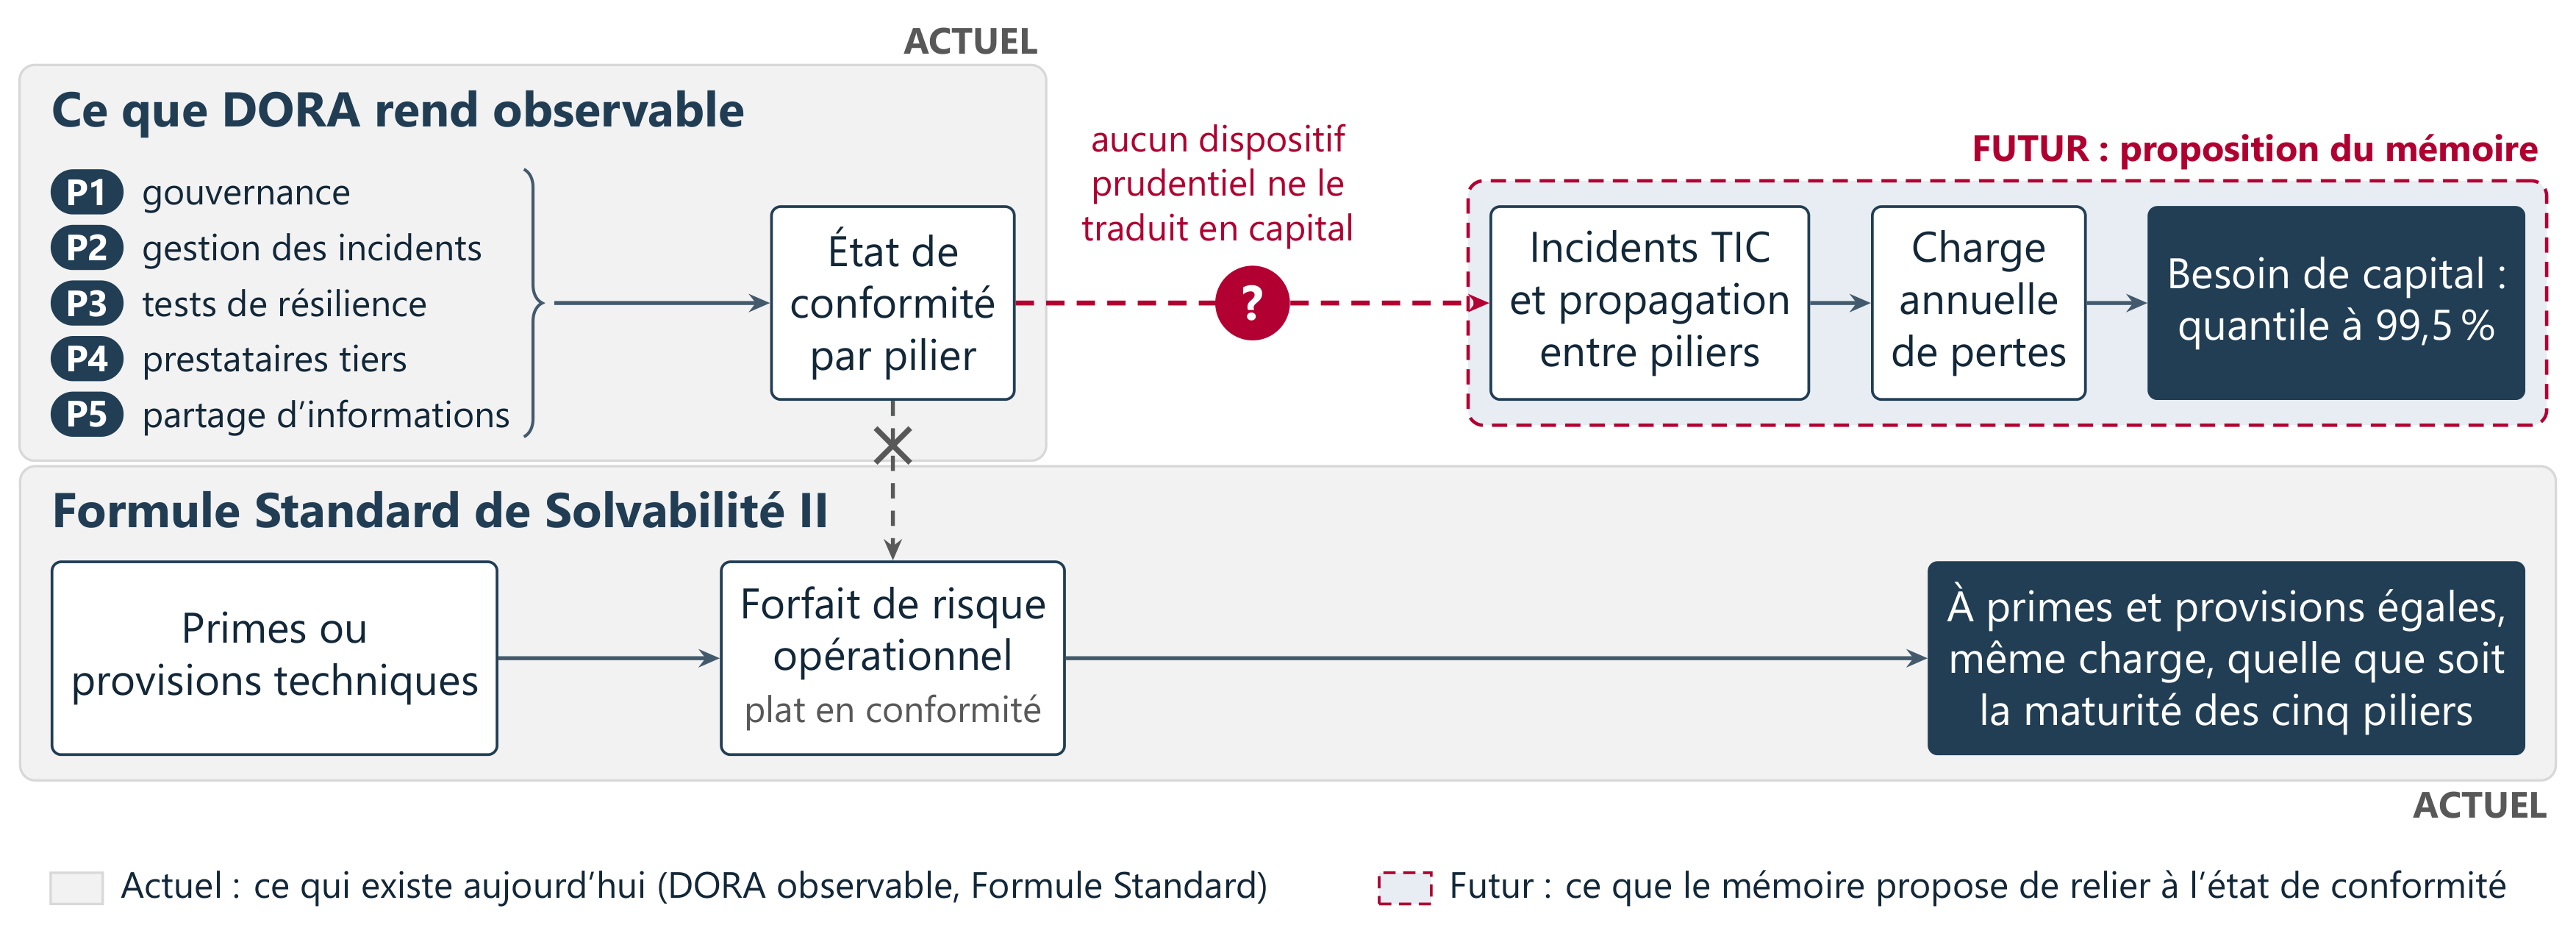
\includegraphics[width=0.90\textwidth]{schema_probleme.png}\\[2mm]
  {\small\color{ardoise}\bfseries Que coûte en capital un défaut de conformité, quel que soit l'état actuel d'une entité ?}
\end{frame}

\begin{frame}{Pourquoi retenir un quantile à 99,5\,\% ?}
  \framesubtitle{\etabli Un repère annuel pour comparer les scénarios de conformité}
  \vspace{-3mm}
  \[B=\VaR_{99{,}5\%}(L),\qquad L=\sum_{n=1}^{N}X_n.\]
  \begin{center}\footnotesize La perte annuelle $L$ additionne les pertes $X_n$ des $N$ incidents survenus dans l'année.\end{center}
  \vspace{3mm}
  \begin{columns}[T,onlytextwidth]
    \column{.30\textwidth}
    {\editorial\normalsize Que représente $B$ ?}\par\vspace{2mm}
    \footnotesize La VaR est un quantile : $B$ est le montant qui couvre les pertes de 99,5\,\% des années du modèle.\par\vspace{2mm}
    Il reste 0,5\,\% d'années où les pertes dépassent ce montant. Ce n'est pas une perte maximale.
    \column{.31\textwidth}
    {\editorial\normalsize Pourquoi 99,5\,\% ?}\par\vspace{2mm}
    \footnotesize On retient le même horizon annuel et le même niveau de confiance que Solvabilité II.\par\vspace{2mm}
    Ce montant sert à l'évaluation interne des risques. Il ne représente pas le capital réglementaire complet de l'entité.\par\vspace{2mm}
    Ce repère ne garantit pas la précision du montant estimé.
    \column{.31\textwidth}
    {\editorial\normalsize\color{accent}Et la CVaR / ES ?}\par\vspace{2mm}
    \footnotesize La CVaR, aussi appelée Expected Shortfall (ES), est la moyenne des 0,5\,\% de pires pertes annuelles. C'est une mesure \textbf{cohérente}, notamment sous-additive.\par\vspace{2mm}
    \textbf{OpRisk ajusté} : $\hat\xi\approx0{,}595<1$, donc ES finie, en complément de la VaR.\par\vspace{2mm}
    \textbf{PRC non plafonnée} : $\hat\xi\approx1{,}033>1$, donc ES infinie.
  \end{columns}
% Reference interne (hors diapositive) : rapport, chapitres 4, 9 et 10. VaR : Value at Risk, quantile de perte. ORSA : évaluation interne des risques et de la solvabilité. SCR : capital de solvabilité requis.
% Reference interne (hors diapositive) : Acerbi et Tasche (2002), On the coherence of Expected Shortfall, arXiv:cond-mat/0104295 ; diagnostic agrege OpRisk : script 73, sortie resultats/sorties_verif/73.txt.
\end{frame}

\begin{frame}{Que propose déjà la littérature, et que lui manque-t-il ?}
  \framesubtitle{Travaux existants et propriétés d'une dépendance entre domaines de contrôle}
  \centering\scriptsize\vspace*{-3mm}
  \renewcommand{\arraystretch}{1.0}
  \setlength{\tabcolsep}{3pt}
  \begin{tabular}{@{}c >{\raggedright\arraybackslash}p{0.285\textwidth} *{5}{>{\centering\arraybackslash}p{0.108\textwidth}}@{}}
    \toprule
    & & \cc{\textbf{Statique}} & \multicolumn{4}{c}{\textbf{Contagion dirigée}} \\
    \cmidrule(lr){3-3}\cmidrule(lr){4-7}
    \textbf{Famille} & \textbf{Travaux} & \cc{\textbf{Dépendance des pertes}} & \cc{\textbf{Direction}} & \cc{\textbf{Ordre d'atteinte}} & \cc{\textbf{Cycles de $W$}} & \cc{\textbf{Propagation}} \\
    \midrule
    \multirow{2}{*}{\raisebox{0pt}[0pt][0pt]{\rotatebox[origin=c]{90}{\textbf{Copules}}}}
      & \auteur{Böhme et Kataria (2006)} & \ck{Copule} & & & & \\
      & \auteur{Herath et Herath (2011)} & \ck{Copule} & & & & \\
    \midrule
    \multirow{4}{*}{\raisebox{0pt}[0pt][0pt]{\rotatebox[origin=c]{90}{\textbf{Dynamique}}}}
      & \auteur{Hillairet et Lopez (2021)} & & \ck{Réseau d'entités} & & \ck{Boucles admises} & \ck{SIR, états} \\
      & \auteur{Hillairet, Lopez et al. (2022)} & & \ck{Réseau d'entités} & & \ck{Boucles admises} & \ck{SIR, portefeuille} \\
      & \auteur{Bessy-Roland et al. (2021)} & & \ck{Types d'attaque} & & \ck{Boucles admises} & \ck{Auto-excitation} \\
      & \auteur{Boumezoued et al. (2023)} & & \ck{Types d'attaque} & & \ck{Boucles admises} & \ck{Excitation ext.} \\
    \midrule
    \multirow{1}{*}{\raisebox{0pt}[0pt][0pt]{\rotatebox[origin=c]{90}{\textbf{Ici}}}}
      & \begin{tabular}[c]{@{}l@{}}\textbf{Ce travail (2026)}\end{tabular} & \ckr{Part $S$} & \ckr{Modélisée} & \ckr{Ordonnés} & \ckr{Admis dans $W$} & \ckr{Entre piliers} \\
    \bottomrule
  \end{tabular}
  \par\vspace{1.5mm}
  \begin{flushleft}\footnotesize\color{ardoise}
  \textbf{Nous gardons} des copules les marges et le risque extrême, de Hillairet et Lopez les états successifs.
  \textbf{Nous ajoutons} une cascade dirigée entre piliers, dont le sens est modélisé, non identifié, puis borné.
  \end{flushleft}
% Reference interne (hors diapositive) : rapport, chapitre 2 (revue de littérature). Ordre d'atteinte : suite des piliers touchés par un incident. Cycles de $W$ : boucles admises dans le graphe.
\end{frame}

% =============================================================================
\section{Données}

\begin{frame}{De quelles données disposons-nous, et que permettent-elles ?}
  \framesubtitle{La fréquence et la sévérité des pertes extrêmes, pas la direction de la contagion}
  \begin{columns}[T]
    \column{0.70\textwidth}
    \scriptsize
    \renewcommand{\arraystretch}{1.3}
    \begin{tabularx}{\linewidth}{>{\hsize=0.85\hsize}Y >{\hsize=1.0\hsize}Y >{\hsize=1.1\hsize}Y >{\hsize=1.05\hsize}Y}
      \toprule
      \textbf{Source} & \textbf{Effectif retenu} & \textbf{Rôle dans le modèle} & \textbf{Biais et limites} \\
      \midrule
      \textbf{SAS OpRisk Global} & 41\,975 pertes, dont 582 cyber × finance & Sévérité en euros ; fréquence d'entrée du moteur & Sélection : biais vers les grandes entités \\
      \rowcolor{clair}\textbf{Chronologie PRC} & 15\,053 incidents, 2019 à 2025 & Fréquence de référence, sans rôle de niveau & Mesure : sévérité dérivée d'un modèle log-log \\
      \textbf{Hackmageddon} & 1\,041 incidents, premier semestre 2026 & Parts par vecteur d'attaque & Déclaration : incidents publics, taxonomie instable \\
      \bottomrule
    \end{tabularx}\\[3mm]
    \small Le niveau de fréquence est lu sur OpRisk, la répartition par vecteur d'attaque sur Hackmageddon.
    Aucune de ces sources ne dit quel pilier a entraîné l'autre : la direction de la contagion n'y est pas observée.
    \question{Comment relier ces pertes à l'état de conformité de chaque pilier ?}
    \column{0.26\textwidth}
    \chiffre{582 pertes / 91 excès}{Base étendue décrite dans le rapport, dont douze pertes antérieures à 2000.}
    \vspace{2mm}
    \chiffre{570 pertes / 86 excès}{Filtre 2000--2026 : échantillon des compléments après dépôt, aux slides 10 et 11. Seuil commun : 20,03 M€.}
    \vspace{4mm}
    \chiffre{1 sinistre}{au-delà de 10\Meur sur le marché français en 2025 : la sévérité se calibre sur une base internationale}
  \end{columns}
\end{frame}

% =============================================================================

\section{Modèle}

\begin{frame}[t]{Comment relier la conformité au capital ?}
  \framesubtitle{Quatre canaux ; paramètres de conformité posés (chapitres 4 à 6) ; cadres rouges : ajouts}
  \centering
  \resizebox{\linewidth}{!}{%
  \begin{tikzpicture}[x=1mm,y=1mm,
    bloc/.style={draw=nexialog!65,fill=white,align=center,inner sep=1mm,
      font=\fontsize{6.5}{7.6}\selectfont},
    canal/.style={fill=nexialog,text=white,rounded corners=.5mm,
      align=center,text width=23mm,inner sep=1mm,font=\fontsize{7}{8.2}\selectfont},
    flux/.style={-{Stealth[length=1.3mm]},draw=nexialog!75,line width=.6pt}]
    \path[use as bounding box] (0,-55) rectangle (146,0);
    % 1 : état latent et deux seuils, comme dans le croquis.
    \node[bloc,draw=accent,line width=.9pt,minimum width=28mm,minimum height=54mm] (etat) at (14,-27) {};
    \node[align=center,font=\fontsize{7}{8.2}\selectfont,text=nexialog] at (14,-5.5)
      {\textbf{1 · État de conformité}\\pour chaque pilier};
    \node[font=\fontsize{7}{8.2}\selectfont] at (14,-12.5)
      {$C^\star=\gamma\Theta+\sqrt{1-\gamma^2}\,\varepsilon$};
    \draw[nexialog!60,->] (2,-19)--(26,-19);
    \foreach \x/\lab in {10/{$K_{\rm bas}$},18/{$K_{\rm haut}$}}{
      \draw[nexialog] (\x,-18)--(\x,-20);
      \node[below,font=\fontsize{5.5}{6}\selectfont] at (\x,-20) {\lab};}
    \foreach \x/\lab in {5/NC,14/PC,23/C}
      \node[font=\fontsize{6}{7}\selectfont,text=nexialog] at (\x,-16.5) {\lab};
    \draw[filet] (3,-26)--(25,-26);
    \node[anchor=north west,align=left,text width=24.5mm,inner sep=0pt,font=\fontsize{5.6}{7}\selectfont,text=gris] at (2,-27.5)
      {NC : non conforme\\PC : partiellement conforme\\C : conforme\\[1mm]
       $C^\star$ : capacité latente\\$\Theta$ : facteur commun\\$\varepsilon$ : choc propre\\$\gamma$ : charge du facteur\\$K$ : seuils de classement};
    \begin{uncoverenv}<2->
    % 2 : quatre canaux, alignés avec leurs trois mécanismes.
    \node[bloc,draw=accent,line width=.9pt,fill=nexialog!5,minimum width=27mm,minimum height=54mm] at (46.5,-27) {};
    \node[font=\fontsize{7}{8.2}\selectfont,text=nexialog] at (46.5,-3) {\textbf{2 · Quatre canaux}};
    \node[canal] (lambda) at (46.5,-9) {Fréquence $\lambda$\\moyenne d'incidents/an};
    \node[canal] (pu) at (46.5,-26) {Détection $p_u$\\probabilité de dépasser $u$};
    \node[canal] (gain) at (46.5,-38.5) {Propagation $g$\\intensité des transmissions};
    \node[canal] (acc) at (46.5,-49.5) {Accumulation\\prestataire commun\\(choc commun)};
    \draw[flux] (etat.east)--(33,-27);
    % 3--5 : lois et matrice ; T remplace l'ancien nom de code TRANS.
    \node[bloc,text width=40mm,minimum height=17mm] (freq) at (86,-9) {
      \textcolor{nexialog}{\textbf{3 · Fréquence} (ch. 4)}\\[.6mm]
      $N$ : nombre annuel, loi binomiale négative\\[.8mm]
       $\lambda$ : moyenne ; $\varphi=9{,}20$\\[.5mm]
      $\varphi=\mathrm{Var}(N)/\mathbb E[N]$ : dispersion.};
    \node[bloc,text width=40mm,minimum height=17mm] (sev) at (86,-26.5) {
      \textcolor{nexialog}{\textbf{4 · Sévérité} (ch. 4)}\\[.6mm]
      Excès : Pareto généralisée (GPD)\\[.7mm]
      $\xi$ : forme ; $\sigma$ : échelle des pertes\\[.6mm]
      $Y_k=0$ avec prob. $1-p_u$,\\sinon $u+\mathrm{GPD}(\xi,\sigma)$ ; $u=20{,}03$ M€.};
    \node[bloc,draw=accent,line width=.9pt,text width=40mm,minimum height=20mm] (casc) at (86,-45) {
      \textcolor{nexialog}{\textbf{5 · Cascade dirigée} (ch. 5)}\\[.7mm]
      $W=g\,\dfrac{T}{\max_j\sum_k T_{jk}}$\\[.7mm]
      $T$ : forces des liens ; $W$ : probabilités.\\
      $S_a$ : piliers touchés depuis l'amorce $a$.\\
      \textcolor{accent}{Accumulation : si l'amorce est P4, un choc commun touche les autres piliers.}};
    \draw[flux] (lambda.east)--(freq.west);
    \draw[flux] (pu.east)--(sev.west);
    \draw[flux] (gain.east)--([yshift=3mm]casc.west);
    \draw[flux] (acc.east)--([yshift=-3mm]casc.west);
    \end{uncoverenv}
    \begin{uncoverenv}<3->
    % 6--7 : un bloc final commun, rouge Nexialog comme dans la référence.
    \node[bloc,draw=accent,fill=accent,text=white,text width=27mm,minimum height=35mm] (cap) at (131,-27) {
      \textbf{6–7 · Pertes et capital}\\[2mm]
      $X_n=\displaystyle\sum_{k\in S_a}Y_{n,k}$\\[1mm]
      perte d'un sinistre\\[2mm]
      $\VaR_{99{,}5\%}\!\left(\displaystyle\sum_{n=1}^{N}X_n\right)$\\[1mm]
      quantile de la charge\\annuelle agrégée};
    \draw[flux] (freq.east)--node[above,font=\scriptsize] {$N$} ([yshift=11mm]cap.west);
    \draw[flux] (sev.east)--node[above,font=\scriptsize] {$Y_k$} (cap.west);
    \draw[flux] (casc.east)--node[below,font=\scriptsize] {$S_a$} ([yshift=-11mm]cap.west);
    \node[align=center,font=\fontsize{6}{7.2}\selectfont,text=nexialog] (ent) at (131,-51)
      {\textbf{8 · À l'échelle d'une entité}\\$A$ : actifs ; $m(A)$ : facteur de perte};
    \draw[flux] (cap.south)--(ent.north);
    \end{uncoverenv}
  \end{tikzpicture}}
% Reference interne (hors diapositive) : rapport, chapitres 4 à 6 et 9. États et écarts entre états supposés ; capital de scénario, niveau illustratif.
\end{frame}

\begin{frame}{Comment l'état règle-t-il la propagation ?}
  \suivimethode{1,2,5}{État et propagation}
  \framesubtitle{\ajout État de conformité $\longrightarrow$ gain $g$ $\longrightarrow$ matrice $W$}
  \begin{columns}[T,onlytextwidth]
  \column{.47\textwidth}\small
  \textbf{1 · Construire l'état}
  \[C^\star=\gamma\Theta+\sqrt{1-\gamma^2}\,\varepsilon\]
  $\Theta$ : facteur commun ; $\varepsilon$ : choc propre, normales centrées réduites indépendantes.\par\vspace{.5mm}
  $\gamma=0{,}68$ : charge du facteur commun.\par\vspace{.5mm}
  $U=\Phi(C^\star)$ : score uniforme, $\Phi$ loi normale standard.\par\vspace{2mm}
  \centering
  \begin{tikzpicture}[x=1mm,y=1mm]
  \fill[accent] (0,0) rectangle (19.6,6);
  \fill[acier] (19.6,0) rectangle (39.2,6);
  \fill[nexialog] (39.2,0) rectangle (56,6);
  \foreach \x/\l in {9.8/NC,29.4/PC,47.6/C}
    \node[text=white,font=\small\bfseries] at (\x,3) {\l};
  \foreach \x/\l in {0/0,19.6/{0,35},39.2/{0,70},56/1}
    \node[below,font=\footnotesize] at (\x,-0.5) {\l};
  \end{tikzpicture}\par\vspace{1.5mm}
  {\footnotesize NC non conforme · PC partiellement conforme · C conforme}
  \column{.49\textwidth}\small
  \textbf{2 · Associer un gain posé}\par\vspace{2mm}
  \centering
  \renewcommand{\arraystretch}{1.4}
  \setlength{\tabcolsep}{4mm}
  \begin{tabular}{@{}l ccc@{}}
    & \cellcolor{accent}\textcolor{white}{\bfseries NC} & \cellcolor{acier}\textcolor{white}{\bfseries PC}
      & \cellcolor{nexialog}\textcolor{white}{\bfseries C} \\
    $g$ & \cellcolor{clair}0,90 & \cellcolor{clair}0,68 & \cellcolor{clair}0,45 \\
  \end{tabular}\par\vspace{4mm}
  \raggedright
  \textbf{3 · Normaliser la propagation}\par\vspace{1.5mm}
  \begin{beamercolorbox}[wd=\linewidth,rounded=true,sep=2mm]{block body example}
  \centering $W=g\,\dfrac{T}{s_{\max}},\qquad s_{\max}=\max_j\sum_k t_{jk}$\par\vspace{2mm}
  \raggedright\footnotesize
  $T=(t_{jk})$ : force posée du lien $j\to k$\par
  $s_{\max}=2{,}6$ : émission maximale\par
  $W_{jk}$ : probabilité de transmission\par\vspace{1mm}
  Chaque ligne somme à au plus $g<1$, donc $\rho(W)\le g$.
  \end{beamercolorbox}
  \end{columns}
\end{frame}

\begin{frame}{Comment modéliser les pertes rares ?}
  \suivimethode{3,4}{Fréquence et sévérité}
  \framesubtitle{\etabli Tester la loi de comptage, puis ajuster les pertes extrêmes}
  \begin{columns}[T,onlytextwidth]
    \column{.31\textwidth}\scriptsize
    Poisson : variance = moyenne.\par
    Binomiale négative : variance $>$ moyenne.\par\vspace{1mm}
    \textbf{Test du rapport de vraisemblance}\par
    14\,944 cellules firme-année (2005--2022).\par
    $\mathrm{LR}=130{,}5$, \quad $p\approx10^{-30}$.\par\vspace{1mm}
    \textcolor{accent}{Binomiale négative retenue.}
    \column{.66\textwidth}
    \begin{minipage}[t]{.485\linewidth}\centering
      {\scriptsize\bfseries Vie résiduelle moyenne $e(v)$, M€\\[-.3mm]\mdseries linéaire au-delà de $u$\par}\vspace{.5mm}
      \adjustbox{trim={.1\width} 0pt 0pt {.22\height},clip,width=.56\linewidth}{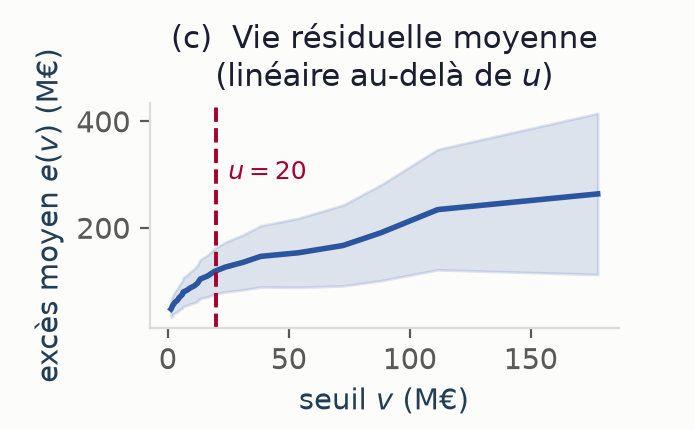
\includegraphics{j3_c.png}}
    \end{minipage}\hfill
    \begin{minipage}[t]{.485\linewidth}\centering
      {\scriptsize\bfseries Stabilité de $\hat\xi$ au seuil\\[-.3mm]\mdseries intervalle à 90\,\%\par}\vspace{.5mm}
      \adjustbox{trim=0pt 0pt 0pt {.165\height},clip,width=.56\linewidth}{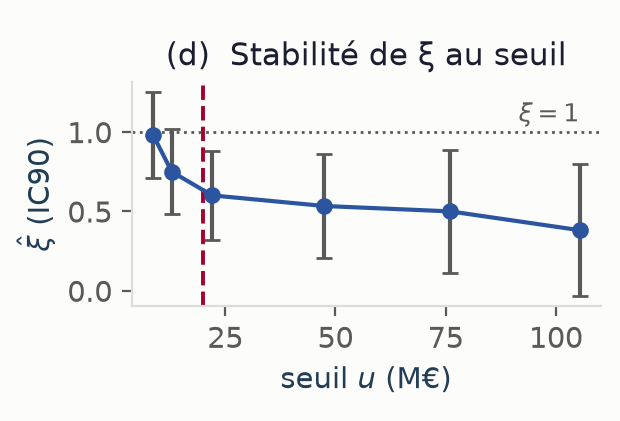
\includegraphics{j3_d.png}}
    \end{minipage}
  \end{columns}
  \vspace{0mm}
  \centering\footnotesize
  {\scriptsize\textbf{Sévérité : loi de Pareto généralisée (GPD).} Complément après dépôt : 570 pertes, 86 excès, 2000--2026.\par}
  \renewcommand{\arraystretch}{1.1}
  \begin{tabular}{@{}l c c c c c@{}}
    \toprule
    \textbf{Estimateur} &$\hat\xi$ & IC 95\,\% de $\xi$ & $\hat\sigma$ (M€) & \textbf{Quantile 99,5\,\%} (M€) & IC 95\,\% du quantile \\
    \midrule
    EMV & 0,595 & [0,252 ; 0,897] & 57,98 & \textcolor{accent}{\textbf{663}} & [377 ; 1\,152] \\
    PWM & 0,505 & [0,254 ; 0,622] & 61,50 & 579 & [370 ; 804] \\
    Hill & 1,402 & [1,208 ; 1,605] & --- & --- & --- \\
    Moments & 0,863 & [0,498 ; 1,092] & --- & --- & --- \\
    \bottomrule
  \end{tabular}\par\vspace{.3mm}
  {\scriptsize\color{gris}Le test de fréquence suppose les cellules indépendantes ; il ne calibre pas la dispersion de 9,2 posée dans le moteur.\par}
  {\scriptsize\color{gris}EMV : maximum de vraisemblance ; PWM : moments pondérés. Quantiles par sinistre, \textbf{pas des capitaux annuels}.\par}
  {\scriptsize Quantile \textbf{robuste} à 95\,\% : 1\,037 M€, borne haute de l'intervalle à 90\,\%.\par}
% Reference interne (hors diapositive) : rapport, chapitre 4 ; estimateurs et IC à 95\,\% : script 129, complément après dépôt.
% Reference interne (hors diapositive) : rapport ENSAE, chapitre 4 ; test de frequence : script 47, sortie 47.txt, cellules firme-annee 2005--2022.
\end{frame}

\begin{frame}{Comment choisir le seuil ?}
  \suivimethode{4}{Seuil de la sévérité}
  \framesubtitle{\etabli 2000--2026 : 570 pertes, 86 excès}
  \begin{columns}[T,onlytextwidth]
    \column{.58\textwidth}
    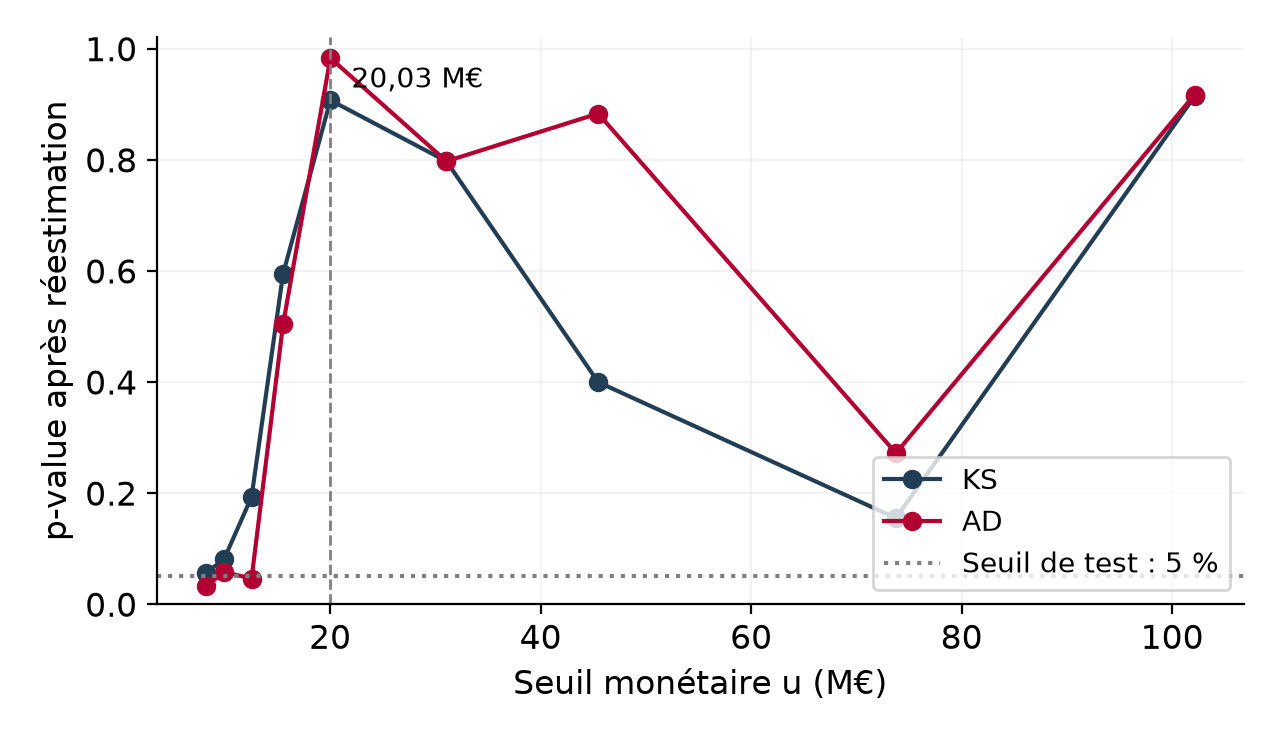
\includegraphics[width=\linewidth]{../../vasicek_lab/figures_inst/G129_tests_seuils.png}
    \column{.38\textwidth}\small
    \textbf{Diagnostic}\par\vspace{1mm}
    Kolmogorov-Smirnov (KS) et Anderson-Darling (AD) : p-value après réestimation, pour neuf seuils candidats.\par\vspace{2mm}
    Au seuil de \textbf{20,03 M€}, elles valent 0,91 (KS) et 0,98 (AD).\par\vspace{2mm}
    Les diagnostics évaluent la compatibilité avec la GPD, sans établir un optimum.\par\vspace{2mm}
    Hill dépasse l'estimateur du maximum de vraisemblance : un écart que la simulation reproduit sous $\xi=0{,}595$ (rapport, chapitre 4).
  \end{columns}
% Reference interne (hors diapositive) : script 129, complément après dépôt. KS : Kolmogorov-Smirnov ; AD : Anderson-Darling. EMV : maximum de vraisemblance. Estimateurs et IC : tableau de la diapositive précédente.
\end{frame}





\begin{frame}{Comment un choc gagne-t-il les autres piliers ?}
  \suivimethode{5}{Propagation du choc}
  \framesubtitle{\ajout Du Vasicek à un facteur à une contagion dirigée entre piliers}
  \centering
  \vspace{1mm}
  \resizebox{\linewidth}{!}{%
  \begin{tikzpicture}[x=1mm, y=1mm, font=\fontsize{6.6}{8}\selectfont,
      bt/.style={anchor=north west, align=center, inner sep=1.6mm, rounded corners=2pt, line width=0.6pt,
                 minimum height=31mm},
      lien/.style={->, line width=0.9pt, draw=acier}]
    \node[bt, draw=gris!60, fill=clair, text width=36mm] (v) at (0,0) {%
      {\bfseries\color{ardoise} Vasicek à un facteur}\\[0.3mm]
      {\color{gris} le modèle de crédit de départ}\\[1.8mm]
      $X_i=\sqrt{\rho}\,Y+\sqrt{1-\rho}\,\varepsilon_i$\\[1.2mm]
      $Y$ : facteur systémique, $\mathcal N(0,1)$\\
      $\varepsilon_i$ : choc propre, $\mathcal N(0,1)$\\[1mm]
      Défaut si $X_i\ge K_i$\\
      $K_i=\Phi^{-1}(1-\mathrm{PD}_i)$};
    \node[bt, draw=accent, fill=white, text width=66mm] (f) at (42,0) {%
      {\bfseries\color{accent} Extension : un facteur par pilier, et la contagion}\\[1.8mm]
      $X_{ij}=\underbrace{\textstyle\textcolor{accent}{\sum_{k\neq j}W_{kj}\,X_{ik}}}_{\textcolor{accent}{\text{contagion } k\to j}}
        +\sqrt{\rho_{ij}}\,Y_{j}+\sqrt{1-\rho_{ij}}\,\varepsilon_{ij}$\\[1.5mm]
      Forme réduite sur les cinq piliers :\\[.6mm]
      $\mathbf X_i=\textcolor{accent}{(I-W^{\top})^{-1}}\,(\text{systémique}+\text{idiosyncratique})$\\[.8mm]
      \textcolor{accent}{$I-W^{\top}$ est inversible car $\rho(W)<1$} ($\rho(W)=0{,}506$ à $g=0{,}90$)};
    \node[bt, draw=gris!60, fill=clair, text width=36mm] (s) at (114,0) {%
      {\bfseries\color{accent} Seuil d'incident}\\[0.3mm]
      {\color{gris} substitut de $\Phi^{-1}(1-\mathrm{PD})$, par pilier}\\[1.8mm]
      Incident sur $j$ si $X_{ij}\ge K_j$\\[1mm]
      $K_j=F_{\text{latent}}^{-1}(1-p_j)$\\[1mm]
      $p_j$ : probabilité cible de dépassement du stress du pilier $j$};
    \draw[lien] (v.east) -- (f.west);
    \draw[lien] (f.east) -- (s.west);
  \end{tikzpicture}}\par\vspace{2.5mm}
  \raggedright\footnotesize
  Le cadre individuel serait $K_{ij}=F_{ij}^{-1}(1-p_{ij})$ : $F_{ij}$ est la fonction de répartition continue du stress
  de l'entité $i$, pilier $j$, et $p_{ij}$ sa probabilité cible de dépassement.\par\vspace{1mm}
  Les données ne permettent pas d'identifier ces marges et probabilités individuelles : nous retenons une loi latente
  de référence commune pour ce cadre de stress.\par\vspace{1.5mm}
  \textbf{Calcul du capital :} le moteur simule directement fréquence, cascade et sévérité ; il n'utilise pas les seuils $K_{ij}$.
% Reference interne (hors diapositive) : rapport, chapitre 5. $i$ : entité ; $j,k$ : piliers ; $W_{kj}$ : du pilier $k$ vers $j$.
\end{frame}








% =============================================================================

\section{Identifiabilité}

\begin{frame}{Peut-on identifier le sens de la propagation ?}
  \suivimethode{5}{Direction des liens}
  \framesubtitle{\ajout $S$ est symétrique ; $A$ est antisymétrique et mesure le déséquilibre des sens}
  \only<1>{%
  \vspace{2mm}
  {\centering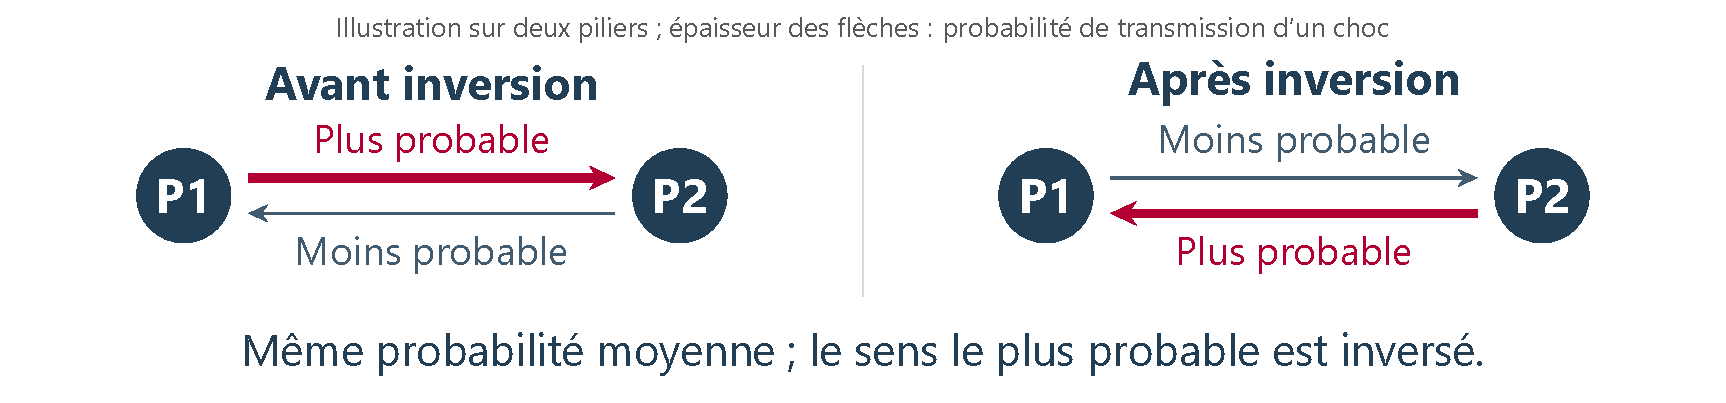
\includegraphics[width=.98\textwidth]{schema_identifiabilite_ensae.pdf}\par}
  \vspace{2mm}
  \begin{columns}[T,onlytextwidth]
    \column{.47\textwidth}\footnotesize
    \textbf{$S$ : partie symétrique.}\par
    Même probabilité moyenne de transmission d'un choc de P1 vers P2 et de P2 vers P1.
    \column{.49\textwidth}\footnotesize
    \textbf{$A$ : partie antisymétrique.}\par
    Elle mesure si P1 transmet plus facilement un choc à P2, ou l'inverse.
  \end{columns}\vspace{2mm}
  \footnotesize Dans l'application, $S$ est posé et l'on fait varier $A$ : la direction reste non identifiée.}
  \only<2->{%
  \vspace{3mm}
  \begin{columns}[T,onlytextwidth]
    \column{.52\textwidth}
    \small\textbf{$S$ : partie symétrique}\par\vspace{2mm}
    \footnotesize Pour deux piliers, elle retient la moyenne des probabilités de transmission d'un choc et l'attribue aux deux sens : de P1 vers P2 et de P2 vers P1.\par\vspace{4mm}
    \small\textbf{$A$ : partie antisymétrique}\par\vspace{2mm}
    \footnotesize Elle mesure la moitié de l'écart entre ces probabilités. Elle précise si P1 transmet plus facilement un choc à P2, ou si P2 le transmet plus facilement à P1.\par\vspace{4mm}
    Inverser les liens conserve $S$, mais inverse le déséquilibre décrit par $A$.
    \column{.43\textwidth}
    \small\textbf{Sur le réseau à cinq piliers}\par\vspace{1.5mm}
    Inverser le sens des liens
    conserve la probabilité moyenne entre chaque paire de piliers et le rayon spectral (0,506), mais change la propagation.\par\vspace{4mm}
    \footnotesize
    Après inversion, la part de sinistres multi-piliers passe de $62{,}31\,\%$ à $50{,}77\,\%$ et le premier pilier à remédier de P1 à P4.\par\vspace{4mm}
    {\scriptsize Gain de propagation : 0,90 ; cascade seule, hors choc commun P4. Retourner la matrice déplace le capital de $3{,}6\,\%$ (295\Meur) ; l'écart atteint 1\,173\Meur{} sur l'ensemble admissible.\par}
    \vspace{2mm}{\scriptsize L'équivalence au premier ordre suppose une amorce uniforme et une faible intensité.\par}
  \end{columns}}
% Reference interne (hors diapositive) : rapport, chapitres 5, 7 et 8. Lecture de la co-occurrence au premier ordre : amorce uniforme, faible intensité. $S$ est posé à dire d'expert dans l'application.
\end{frame}





\begin{frame}{1 · Quelles directions faut-il envisager ?}
  \suivimethode{5}{Matrices candidates}
  \framesubtitle{\ajout Un choix de direction pour chaque paire de piliers}
  \vspace{2mm}
  \begin{columns}[T,onlytextwidth]
  \column{.34\textwidth}\centering
  \begin{tikzpicture}[scale=0.95]
    \foreach \n/\a in {1/90,2/18,3/-54,4/-126,5/162}
      \node[pilier] (P\n) at (\a:1.5) {P\n};
    \foreach \i/\j in {1/2,1/3,1/4,1/5,2/3,2/4,2/5,3/4,3/5,4/5}
      \draw[acier] (P\i)--(P\j);
    \draw[fla] (P1)--(P2);
    \node[font=\scriptsize,text=accent,align=center] at (0,-2.35) {chaque arête : un sens à choisir};
  \end{tikzpicture}
  \column{.62\textwidth}\small
  \textbf{Compter.}
  \[\underbrace{\frac{5\times4}{2}=10}_{\text{paires}}\quad\longrightarrow\quad
  \textcolor{accent}{\underbrace{2^{10}=1\,024}_{\text{configurations de signes}}}\]
  \textbf{Construire.} $A_{jk}=\varepsilon_{jk}\,t\,S_{jk}$, avec $\varepsilon_{jk}\in\{-1,+1\}$ et $A_{kj}=-A_{jk}$.\par
  $t$ : amplitude d'asymétrie ; $S$ reste fixé.\par\vspace{2mm}
  \textbf{Filtrer.} Garder $W=S+A$ tel que
  \[0\le W_{jk}\le1,\qquad\rho(W)<1.\]
  {\footnotesize\color{gris}Ces configurations diffèrent des $5!=120$ ordres des cinq piliers.}
  \end{columns}
% Reference interne (hors diapositive) : rapport, chapitre 8. Sommets d'un pavé, puis filtre d'admissibilité ; les extrema globaux ne sont pas démontrés.
\end{frame}


\begin{frame}{2 · Que coûte un incident qui se propage ?}
  \suivimethode{4,5,6}{Perte par incident}
  \framesubtitle{Une amorce, des transmissions indépendantes, une sévérité par pilier touché}
  \begin{center}
  \begin{tikzpicture}[node distance=4mm]
    \node[etape] (e1) {\textbf{1. Amorce}\\ Pilier tiré selon les poids de fréquence};
    \node[etape, right=of e1] (e2) {\textbf{2. Transmissions}\\ Chaque arête $j\to k$ avec probabilité $W_{jk}$};
    \node[etape, right=of e2] (e3) {\textbf{3. Ensemble atteint}\\ $S_a$ : piliers touchés, comptés une fois};
    \node[etape, right=of e3] (e4) {\textbf{4. Perte}\\ $X=\sum_{k\in S_a} Y_k$};
    \draw[fl] (e1) -- (e2); \draw[fl] (e2) -- (e3); \draw[fl] (e3) -- (e4);
  \end{tikzpicture}
  \end{center}
  
  \begin{center}
    \centering
    \begin{tikzpicture}[xscale=1.55,yscale=0.85]
      \node[pilier touche] (P1) at (0,1.5) {P1};
      \node[pilier touche] (P2) at (2.0,1.5) {P2};
      \node[pilier] (P3) at (3.8,1.5) {P3};
      \node[pilier touche, fill=accent, draw=accent] (P4) at (1.0,0) {P4};
      \node[pilier] (P5) at (2.9,0) {P5};
      \draw[fla] (P4) -- (P1); \draw[fla] (P4) -- (P2);
      \draw[flnon] (P2) -- (P3); \draw[flnon] (P4) -- (P5);
      \node[font=\scriptsize, text=accent, below=0.5mm of P4] {Amorce};
    \end{tikzpicture}\\[0.5mm]
    {\scriptsize Rouge : transmission réalisée. Pointillés : transmission non réalisée.}
  \end{center}
  \vspace{-0.5mm}
  {\footnotesize Les bornes utilisent la cascade indépendante ; les capitaux par état, la marche auto-évitante.
  Seule la première reste définie si une ligne de $W$ somme à plus de un. Le changement déplace le besoin du secteur
  de $-4\,\%$ : les deux résultats ne se comparent pas directement.\par}
% Reference interne (hors diapositive) : rapport, chapitres 4, 5 et 8.
\end{frame}

\begin{frame}{3 · Que vaut le capital aux 1\,024 sommets ?}
  \suivimethode{7}{Capital aux sommets}
  \framesubtitle{\ajout Un capital par matrice candidate ; la plage est lue sur les sommets}
  \begin{columns}[T,onlytextwidth]
  \column{.67\textwidth}
  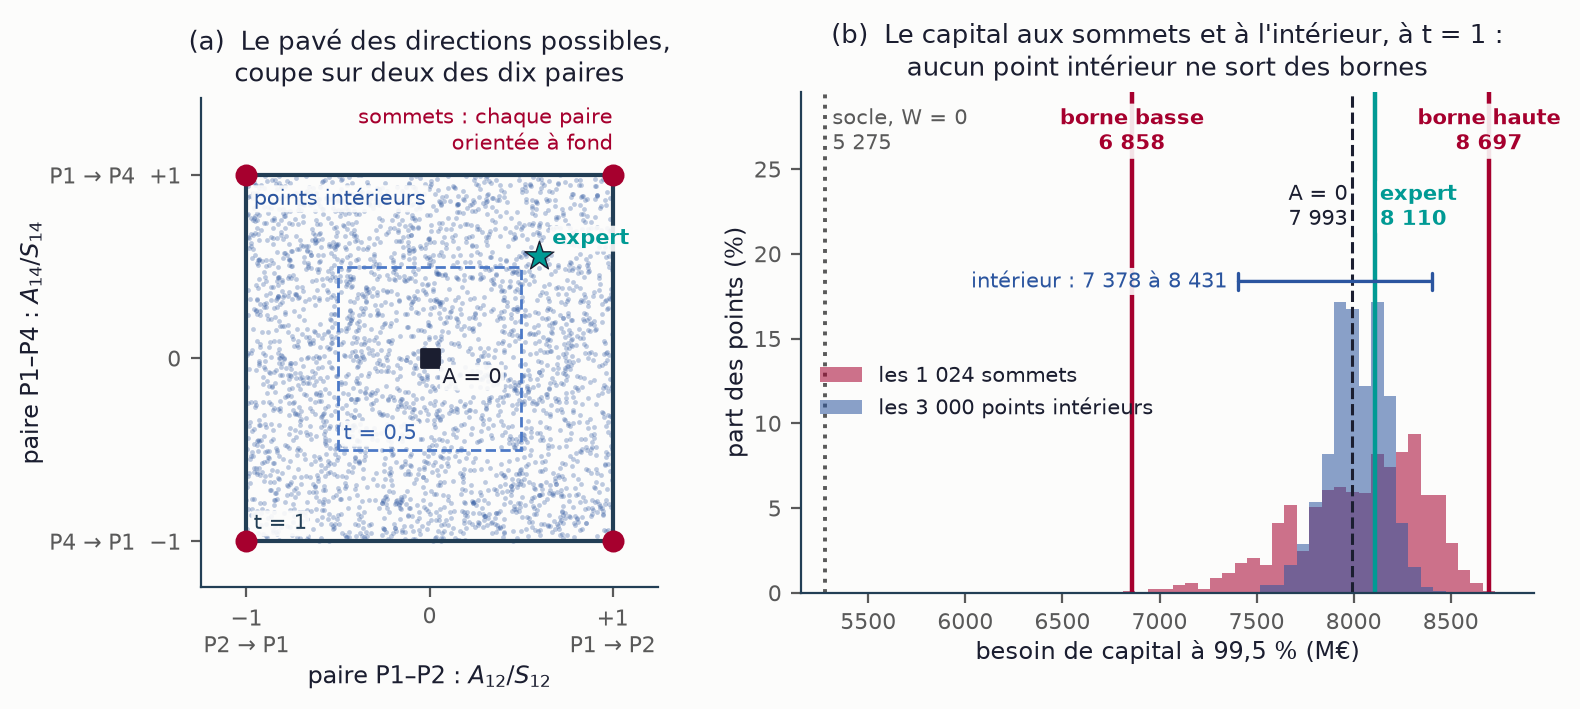
\includegraphics[width=\linewidth]{Z_pave_sommets.png}\par
  {\tiny\color{gris}(a) coupe du pavé sur deux des dix paires. (b) capital aux sommets (rouge) et aux points intérieurs (bleu).\par}
  \column{.30\textwidth}\footnotesize
  \textbf{1 · Simuler une fois}\par
  Mêmes 40\,000 années pour toutes les matrices : les écarts viennent de $W$.\par\vspace{1.5mm}
  \textbf{2 · Un capital par sommet}\par
  $\VaR_{99{,}5\,\%}(L\mid W)$ pour les 1\,024 matrices.\par\vspace{1.5mm}
  \textbf{3 · Lire la plage}\par
  Minimum et maximum sur les sommets ; aucun des 3\,000 points intérieurs n'en sort.\par\vspace{1.5mm}
  {\color{accent}\textbf{[6\,858 ; 8\,697] M€}}, largeur 1\,839 M€.\par\vspace{1mm}
  {\scriptsize\color{gris}Cascade indépendante, fréquence conforme, $g=0{,}90$ : la plage ne se compare pas directement aux capitaux par état (marche auto-évitante).\par}
  \end{columns}
% Reference interne (hors diapositive) : rapport, § 8.1–8.2, figure 9.1. $S$ posée, fréquence conforme, $g=0{,}90$. Extrema globaux non démontrés.
\end{frame}

% =============================================================================

\section{Résultats}

\begin{frame}{Comment mesurer l'effet de la conformité ?}
  \suivimethode{2,7}{Deux états}
  \framesubtitle{\ajout État de conformité, perte annuelle simulée, puis quantile à 99,5\,\%}
  \begin{columns}[T,onlytextwidth]
    \column{.58\textwidth}\footnotesize
    \renewcommand{\arraystretch}{1.3}
    \begin{tabularx}{\linewidth}{@{}l Y r r@{}}
      \toprule
      \textbf{Canal} & \textbf{Paramètre} & \textbf{C} & \textcolor{accent}{\textbf{NC}} \\
      \midrule
      Fréquence & $\lambda$ : incidents par an & 21,56 & \textcolor{accent}{53,62} \\
      Détection & $p_u$ : dépassement de $u$ & 0,128 & \textcolor{accent}{0,181} \\
      Propagation & $g$ : gain de $W$ & 0,45 & \textcolor{accent}{0,90} \\
      Accumulation & probabilité de choc commun & 0 & \textcolor{accent}{0,68} \\
      \bottomrule
    \end{tabularx}\par\vspace{2mm}
    \textbf{Calcul pour chaque état $e$}
    \setlength{\abovedisplayskip}{1mm}\setlength{\belowdisplayskip}{1mm}
    \setlength{\abovedisplayshortskip}{1mm}\setlength{\belowdisplayshortskip}{1mm}
    \[B_e=\VaR_{99{,}5\,\%}\!\left(\sum_{n=1}^{N_e}X_{n,e}\right).\]
    {\scriptsize $e$ : conforme (C) ou non conforme (NC) ; $N_e$ : incidents annuels ; $X_{n,e}$ : perte de l'incident $n$, après détection, propagation et accumulation.\par\vspace{1mm}
    Même moteur et mêmes graines ; les quatre canaux varient selon $e$.\par\vspace{1mm}}
    {\scriptsize\color{gris}Paramètres non conformes posés, non estimés.}
    \column{.38\textwidth}
    \centering
    \begin{tikzpicture}[x=1mm,y=1mm]
      \draw[filet] (0,0)--(46,0);
      \fill[gris!45] (5,0) rectangle (19,6.6);
      \fill[accent] (27,0) rectangle (41,22);
      \node[above,font=\scriptsize,text=ardoise] at (12,6.6) {6\,049 M€};
      \node[above,font=\scriptsize,text=accent] at (34,22) {20\,188 M€};
      \node[below,font=\scriptsize] at (12,0) {Conforme};
      \node[below,font=\scriptsize] at (34,0) {Non conforme};
    \end{tikzpicture}\par\vspace{1mm}
    {\editorial\fontsize{18}{19}\selectfont\color{accent}$\times\,3{,}34$}\par\vspace{.5mm}
    \raggedright\scriptsize Écart de \textbf{14\,139 M€} ; écart-type Monte-Carlo entre quatre graines : 734 M€.
    Interactions entre canaux : \textbf{35\,\%} de l'écart.\par\vspace{.5mm}
    {\color{accent}Suppose que les pertes des piliers touchés s'additionnent.}
  \end{columns}
% Reference interne (hors diapositive) : rapport, chapitre 6 et § 9.1. Niveau illustratif ; l'amplitude dépend des paramètres posés. Tirages communs seulement entre configurations de même fréquence.
\end{frame}

\begin{frame}{Comment attribuer l'écart à chaque canal ?}
  \suivimethode{2,7}{Attribution par canal}
  \framesubtitle{\ajout Seize configurations, deux lectures d'un même canal}
  \begin{columns}[c,onlytextwidth]
    \column{.56\textwidth}
    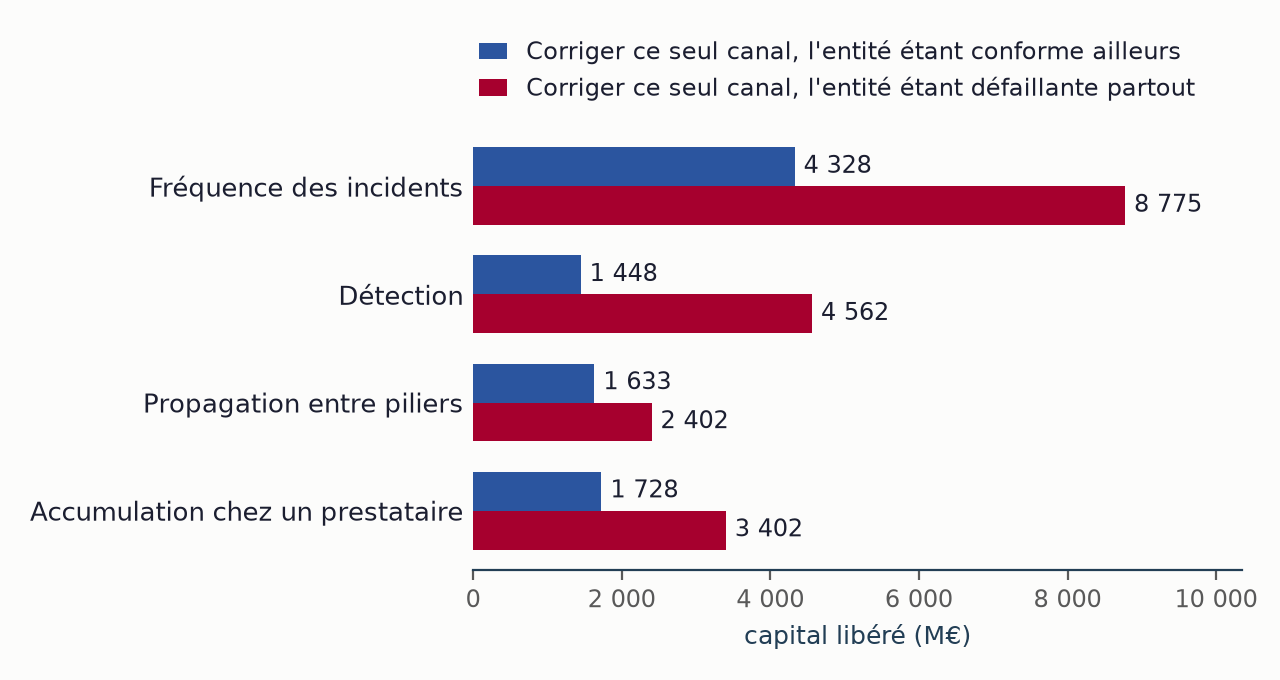
\includegraphics[width=\linewidth]{N1_canaux_note.png}
    \column{.41\textwidth}\footnotesize
    $2^4=16$ configurations, simulées avec les mêmes graines ; $V(\cdot)$ : capital de la configuration.\par\vspace{2mm}
    \textbf{Effet isolé} (depuis l'état conforme)\par
    $\Delta^{\mathrm{iso}}_c=V(\{c\})-V(\varnothing)$\par\vspace{1mm}
    \textbf{Effet de fermeture} (depuis l'état non conforme)\par
    $\Delta^{\mathrm{ferm}}_c=V(\text{tout})-V(\text{tout}\setminus\{c\})$\par\vspace{2mm}
    Fréquence : {\editorial 4\,328 M€} isolé, {\editorial\color{accent}8\,775 M€} en fermeture.
    L'écart entre les deux lectures mesure les interactions que le canal porte.\par\vspace{1mm}
    {\scriptsize\color{gris}Les effets de fermeture ne s'additionnent pas.}\par\vspace{1mm}
    {\small\color{accent}\itshape$\rightarrow$\enspace Et pour une entité donnée ?\par}
  \end{columns}
% Reference interne (hors diapositive) : rapport, chapitre 9, figure 9.1. Gains conditionnels aux paramètres posés ; les gains de fermeture ne s'additionnent pas.
\end{frame}



\begin{frame}{Comment passer du marché à une entité ?}
  \suivimethode{8}{Échelle de l'entité}
  \framesubtitle{Entité notionnelle : adapter les lois, puis recalculer le capital}
  \begin{columns}[T,onlytextwidth]
  \column{.49\textwidth}\footnotesize
  \setlength{\abovedisplayskip}{1mm}\setlength{\belowdisplayskip}{1mm}
  \setlength{\abovedisplayshortskip}{1mm}\setlength{\belowdisplayshortskip}{1mm}
  \textbf{1 · Fréquence à la taille}
  \[\lambda(A)=\lambda_0\Big(\frac{A}{A_0}\Big)^{b_\lambda},\qquad b_\lambda=0{,}494\]
  \textbf{2 · Sévérité à la taille}
  \[m(A)=\Big(\frac{A}{A_m}\Big)^{b},\qquad b=0{,}087\]
  \textbf{3 · Perte et capital de l'entité}
  \[X=m(A)\sum_{k\in S_a}Y_k,\qquad \mathcal B(A)=\VaR_{99{,}5\,\%}\Big(\sum_{n=1}^{N}X_n\Big)\]
  {\scriptsize $A$ : actifs ; $b_\lambda$ estimé sur les firmes de plus de 100 Md\$ (tout le panel : 0,074, fenêtres d'observation plus courtes chez les petites firmes) ;
  $A_m$ : actifs médians des pertes TIC ; pertes sous le seuil incluses ; $N$ : binomiale négative de moyenne $\lambda(A)$.\par}
  \column{.47\textwidth}\footnotesize
  {\scriptsize\color{accent}\textbf{Complément après dépôt : chiffres différents du rapport}\par}\vspace{1mm}
  \renewcommand{\arraystretch}{1.25}
  \begin{tabular}{@{}lrrr@{}}
    \toprule
    \textbf{Entité} & \textbf{Rapport} & \shortstack[r]{\textbf{Nouvelle}\\\textbf{calibration}} & \shortstack[r]{\textbf{Pires}\\\textbf{années}} \\
    \midrule
    Assureur non-vie A & 112 & 1 & 51 \\
    \textbf{Notionnelle} & 169 & \textcolor{accent}{\textbf{24}} & 156 \\
    Assureur vie D & 294 & 193 & 591 \\
    \bottomrule
  \end{tabular}\par\vspace{1mm}
  {\scriptsize En M€. Besoin : quantile à 99,5 \% ; pires années : moyenne des 0,5 \% pires années.\par}\vspace{1mm}
  Notionnelle : bootstrap par firme $[8{,}3\,;53{,}0]$ M€. La baisse vient surtout de la fréquence, et dépend de la dispersion.\par\vspace{2mm}
  {\scriptsize\color{accent}Vise à réduire l'effet des fenêtres courtes ; extrapolation aux petites entités à valider ; métier non intégré.}
  \end{columns}
% Reference interne (hors diapositive) : scripts 136 et 137 (complement apres depot, sorties 136.txt et 137.txt) ; rapport ENSAE, § 9, pour 112, 169 et 294. $W$ et moteur inchanges.
\end{frame}
\section{Bilan}



\begin{frame}{Qu'est-ce que ce stage m'a apporté ?}
  \suivimethode{}{}
  \framesubtitle{Un encadrement exigeant, en entreprise et à l'école}
  \begin{columns}[T]
    \column{.47\textwidth}
    {\editorial\normalsize L'apport de l'encadrement}\par\vspace{3mm}
    \small\textbf{Hugo Rapior · Nexialog Consulting}\par\vspace{1mm}
    Un suivi hebdomadaire et disponible, qui a donné au travail sa rigueur et son ancrage métier.
    Il m'a confié la co-écriture de l'analyse actuarielle de l'étude LUCY 2026, publiée par le cabinet.\par\vspace{3mm}
    \textbf{Caroline Hillairet · ENSAE Paris}\par\vspace{1mm}
    Ses travaux sur les états de conformité et l'excitation des sinistres cyber ont nourri le modèle.
    Ses questions ont fait naître deux briques : le quantile prédictif et la sensibilité aux probabilités de propagation.
    \column{.45\textwidth}
    {\editorial\normalsize Ce que je retiens}\par\vspace{3mm}
    \small Vérifier chaque résultat contre le code qui le produit, du premier calcul au dernier chiffre.\par\vspace{3mm}
    Tracer la calibration et chaque correction, pour qu'un tiers puisse tout refaire.\par\vspace{3mm}
    Séparer ce qui est estimé, supposé et non identifié : c'est ce qui rend un capital défendable.
  \end{columns}
% Reference interne (hors diapositive) : rapport, chapitre « Enseignements du stage ».
\end{frame}

\begin{frame}{Que permet de défendre ce travail ?}
  \suivimethode{}{}
  {\small\color{ardoise}\bfseries Réponse : dans le scénario, la non-conformité multiplie le besoin de capital par 3,34 ;
  la direction de la contagion, non identifiée, est encadrée par une plage explorée aux sommets.\par}
  \vspace{3mm}
  \begin{columns}[T]
    \column{.30\textwidth}
    \chiffre{$\times\,3{,}34$}{Capital entre deux états de conformité supposés}
    \vspace{1.5mm}\footnotesize L'effet est conditionnel aux quatre canaux et à l'addition des pertes entre piliers.
    \column{.30\textwidth}
    \chiffre{1\,839 M€}{Largeur de la plage explorée aux sommets}
    \vspace{1.5mm}\footnotesize Le sens des liens reste non identifié ; la force des liens est posée.
    \column{.30\textwidth}
    {\editorial\normalsize Adapter à l’entité}\par\vspace{2mm}
    \footnotesize Piste à calibrer : adapter la fréquence et les pertes à la taille et au métier, puis recalculer le capital annuel.
  \end{columns}
% Reference interne (hors diapositive) : rapport, chapitres 8 à 10 et conclusion. Résultats conditionnels, niveau absolu illustratif ; extrema globaux non démontrés ; élicitation préparée et diffusée, restée sans réponse.
\end{frame}

{\setbeamertemplate{headline}{}\setbeamertemplate{footline}{}
\begin{frame}[plain]
  \suivimethode{}{}
  \vspace{16mm}\hspace{3mm}{\scriptsize\color{gris}CONFORMITÉ DORA / BESOIN DE CAPITAL}\par
  \vspace{10mm}\hspace{3mm}{\editorial\fontsize{34}{38}\selectfont Merci.}\par
  \vspace{5mm}\hspace{3mm}{\large\color{accent}Place aux questions.}\par
  \vfill\hspace{3mm}{\small Kélian Kaddouri\quad\color{gris}ENSAE Paris · Nexialog Consulting}\par\vspace{8mm}
  \begin{tikzpicture}[remember picture,overlay]
    \node[anchor=south east,inner sep=0pt]
      at ([xshift=-10mm,yshift=18mm]current page.south east)
      {
\includegraphics[height=8mm]{ensae.png}\hspace{5mm}
\includegraphics[height=6mm]{nexialog.png}};
  \end{tikzpicture}
\end{frame}}

% =============================================================================
\end{document}
